\documentclass[11pt]{article}

\usepackage[a4paper,margin=1in]{geometry}
\usepackage{amsmath}
\usepackage{graphicx}
\usepackage{booktabs}
\usepackage{array}
\usepackage{float}
\usepackage[round,authoryear]{natbib}
\usepackage{hyperref}
\usepackage{xcolor}
\usepackage{tikz}
\usetikzlibrary{arrows.meta,positioning}

\hypersetup{
  colorlinks=true,
  linkcolor=black,
  urlcolor=blue,
  citecolor=black
}

\makeatletter
\long\def\@makecaption#1#2{%
  \vskip\abovecaptionskip
  \noindent\textbf{#1}\par
  \noindent\textit{#2}\par
  \vskip\belowcaptionskip}
\makeatother

\title{\textbf{Filipino Adaptation of OmniVoice: Fine-Tuning a Multilingual Text-to-Speech Model Using the Philippine Languages Database}}
\author{COSC-E4 Elective 4 - Machine Learning}
\date{\today}

\begin{document}
\maketitle

\begin{abstract}
This study investigates Filipino adaptation of OmniVoice, a pretrained massively multilingual zero-shot text-to-speech model, using the Filipino subset of the Philippine Languages Database. Although OmniVoice already includes Filipino, the model reports only 7.71 hours of Filipino in its multilingual training mixture, leaving room to examine whether supervised Filipino fine-tuning improves generated speech. The methodology prepares paired Filipino audio and transcript data, filters read-speech utterances, converts the dataset into OmniVoice JSONL and tokenized WebDataset format, fine-tunes the pretrained checkpoint under Kaggle T4 GPU constraints, and evaluates generated audio against the base model. Training and evaluation runs are tracked in Weights and Biases to support hyperparameter comparison across learning rates, step counts, and checkpoint policies. Evaluation uses word error rate for intelligibility, objective speaker similarity for voice cloning quality, and UTMOS for predicted naturalness, with listening checks used to interpret metric changes. The best evaluated checkpoint is the 1e-5 learning-rate run selected by best development loss at step 4900, reducing WER from 22.55\% to 18.52\% while keeping objective speaker similarity slightly above the base model.
\end{abstract}

\section{Introduction}

Text-to-speech (TTS) and voice cloning systems generate speech waveforms from text and, in zero-shot voice cloning settings, imitate a target speaker from a short reference recording. Recent neural speech generation models increasingly use large-scale pretrained models, discrete audio tokens, and generative architectures to synthesize natural and speaker-conditioned speech \citep{valle,voicebox,maskgct,omnivoice}. These systems are useful for accessibility, education, localization, narration, and language-learning tools. However, practical speech generation quality remains uneven across languages because high-resource languages tend to dominate available datasets and benchmarks.

Filipino is widely used in the Philippines, but open Filipino TTS and voice cloning workflows remain less mature than English-focused systems. OmniVoice is a promising starting point because it is open source, supports more than 600 languages, and includes Filipino with language ID \texttt{fil} \citep{omnivoice}. However, language support does not automatically imply strong performance in pronunciation, intelligibility, naturalness, or speaker similarity. The OmniVoice language table lists 7.71 hours of Filipino in its training mixture, while the Philippine Languages Database (PLD) reports 48:56:36 of Filipino speech \citep{pld}. This difference motivates an adaptation study using supervised fine-tuning.

\subsection{Problem Statement}

Open Filipino speech generation systems face two related limitations. First, high-quality voice cloning systems are often optimized around languages with larger training corpora and stronger evaluation coverage. Second, multilingual support in a pretrained model may still be thin for a specific low-resource language, especially when the available language-specific hours are small relative to the full training mixture.

The machine learning problem addressed in this study is:

\begin{quote}
Given a pretrained multilingual TTS model and a curated Filipino speech-text dataset, determine whether supervised fine-tuning improves Filipino speech generation compared with the original base checkpoint.
\end{quote}

The study evaluates improvement using objective metrics for intelligibility, speaker similarity, and naturalness, then interprets those metrics with generated audio samples. The expected outcome is a reproducible fine-tuning and evaluation workflow for measuring Filipino adaptation of OmniVoice.

\section{Related Works}

Voice cloning is closely related to text-to-speech, but its goal is more specific: the system must generate the requested text while preserving the voice characteristics of a target speaker. \citet{voicecloningsurvey} frame modern voice cloning around speaker adaptation, few-shot TTS, zero-shot TTS, and multilingual TTS. This distinction is important for the present study because different settings use different amounts of target data. Speaker adaptation usually updates a model using speaker or language examples, while zero-shot voice cloning tries to imitate a reference voice without updating the model at inference time. This study uses a zero-shot model as its starting point, but the research task itself is supervised adaptation: Filipino text-audio pairs are used to fine-tune the pretrained model.

Recent TTS research has moved from narrowly trained speaker-specific systems toward large pretrained speech generation models. VALL-E helped establish neural codec language modeling for TTS by generating discrete audio codec codes conditioned on text and a short acoustic prompt \citep{valle}. Voicebox extended this direction with text-guided speech infilling and multilingual training, showing that one speech generation model can support several generation and editing tasks \citep{voicebox}. MaskGCT and F5-TTS further reflect the trend toward non-autoregressive generation, where systems aim to produce high-quality speech more efficiently than step-by-step autoregressive decoding \citep{maskgct,f5tts}. Across these works, the shared pattern is clear: modern voice cloning increasingly depends on pretrained generative models, speech tokenizers, and short speaker prompts rather than training a separate model for every speaker.

OmniVoice is the work most directly connected to this project because it combines those trends with broad language coverage. \citet{omnivoice} present OmniVoice as a massively multilingual zero-shot TTS model with a diffusion language model-style, discrete, non-autoregressive architecture. Its main difference from two-stage systems is that it does not first predict semantic tokens and then convert them into acoustic tokens. Instead, OmniVoice directly maps text to multi-codebook acoustic tokens. The model uses full-codebook random masking during training and initializes from pretrained LLM weights to improve intelligibility. It also uses the Higgs Audio tokenizer to extract 8-codebook acoustic tokens and reconstruct speech waveforms \citep{omnivoice,higgsaudio}. These design choices make OmniVoice a practical base model for a Filipino adaptation experiment: the model already supports Filipino, but it can still be tested for improvement when exposed to more Filipino paired speech data.

The machine learning method in this project is supervised fine-tuning, which is a form of transfer learning. Transfer learning reuses knowledge learned from a source setting to improve learning in a related target setting \citep{transferlearning}. In this study, the source setting is OmniVoice's pretrained multilingual speech generation model, and the target setting is Filipino TTS and voice cloning. The supervised labels are the paired PLD transcripts and audio recordings. Fine-tuning is appropriate here because training a modern TTS model from scratch would require far more data and compute than the project constraints allow, while updating a pretrained checkpoint can adapt the text-to-acoustic-token mapping toward Filipino pronunciation and usage under a Kaggle T4 workflow.

The dataset source is the Philippine Languages Database introduced by \citet{pld}. PLD was developed as a multilingual speech corpus for Philippine spoken languages and covers Filipino, English, Cebuano, Kapampangan, Hiligaynon, Ilokano, Bikolano, Waray, and Tausug. The corpus is relevant because it provides the kind of paired speech and transcript data required for supervised TTS fine-tuning. The Filipino subset also gives this study a concrete gap to investigate: OmniVoice already lists Filipino support, but its reported Filipino hours are much smaller than the Filipino speech available in PLD. The project therefore asks whether Filipino-specific supervised adaptation improves the base model instead of assuming that multilingual support alone is sufficient.

Evaluation in recent zero-shot TTS work usually separates three concerns: intelligibility, speaker preservation, and naturalness. Following Voicebox and OmniVoice, this study uses WER or CER for intelligibility, SIM-o for objective speaker similarity, and UTMOS for predicted naturalness \citep{omnivoice,voicebox}. WER and CER are based on edit distance, commonly associated with Levenshtein's insertion, deletion, and substitution operations \citep{levenshtein}. Because WER depends on the ASR model used to transcribe generated speech, this study also cites Whisper, HuBERT, and Paraformer as relevant ASR backends used in modern speech evaluation pipelines \citep{whisper,hubert,paraformer}. Speaker similarity depends on the embedding model, so ECAPA-TDNN and WavLM are included because OmniVoice evaluation uses WavLM-based ECAPA-TDNN speaker embeddings \citep{ecapatdnn,wavlm}. UTMOS is used as an automatic MOS predictor for naturalness \citep{utmos}. Together, these metrics support the main comparison of this project: whether fine-tuned OmniVoice produces Filipino speech that is clearer without losing speaker identity or naturalness.

\section{Objectives}

\subsection{General Objective}

The general objective is to fine-tune and evaluate a pretrained multilingual TTS model for Filipino speech generation using the Philippine Languages Database.

\subsection{Specific Objectives}

\begin{enumerate}
  \item Prepare a clean Filipino read-speech dataset from the Philippine Languages Database.
  \item Convert the prepared dataset into the JSONL and tokenized WebDataset format required by OmniVoice.
  \item Fine-tune the pretrained \texttt{k2-fsa/OmniVoice} checkpoint on Filipino speech using Kaggle T4 GPUs.
  \item Track training and evaluation runs in Weights and Biases for hyperparameter comparison across learning rates, training steps, and checkpoint strategies.
  \item Generate Filipino speech samples from both the base and fine-tuned models using matched test prompts and reference voices.
  \item Evaluate both models using intelligibility, speaker similarity, and naturalness metrics.
  \item Interpret whether Filipino-specific fine-tuning improves generated Filipino speech under limited compute constraints.
\end{enumerate}

\section{System Design and Methodology}

\subsection{System Architecture}

The system has five major stages: dataset preparation, audio tokenization, model fine-tuning, inference, and evaluation.

\begin{figure}[H]
  \centering
  \caption{Fine-tuning and evaluation system architecture.}
  \label{fig:architecture}
  \small
  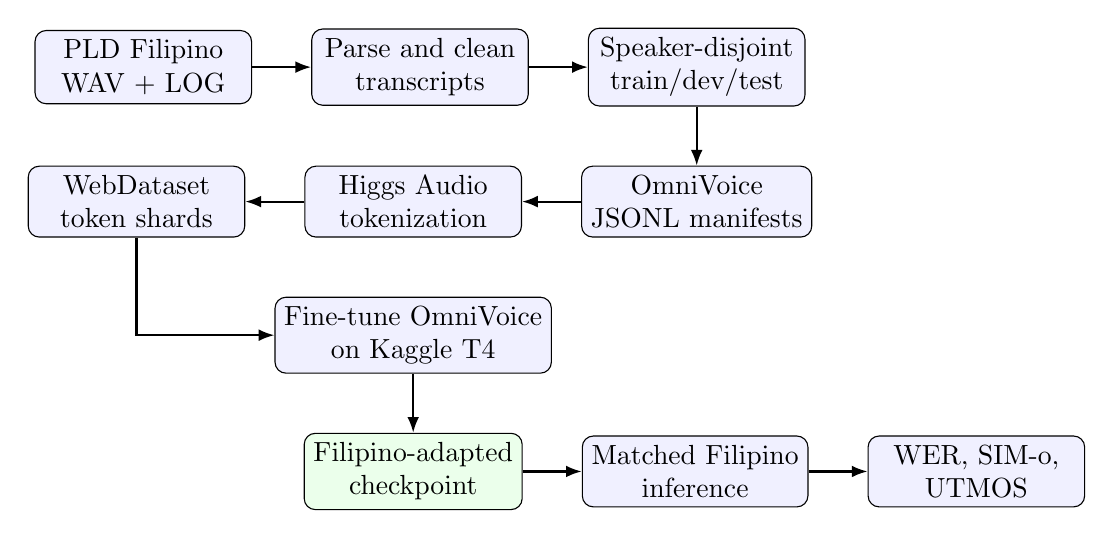
\begin{tikzpicture}[
    node distance=0.75cm and 0.75cm,
    box/.style={draw, rounded corners, align=center, minimum height=0.9cm, minimum width=2.75cm, fill=blue!6},
    outputbox/.style={draw, rounded corners, align=center, minimum height=0.9cm, minimum width=2.75cm, fill=green!8},
    arrow/.style={-{Latex[length=2mm]}, thick}
  ]
    \node[box] (raw) {PLD Filipino\\WAV + LOG};
    \node[box, right=of raw] (parse) {Parse and clean\\transcripts};
    \node[box, right=of parse] (split) {Speaker-disjoint\\train/dev/test};
    \node[box, below=of split] (jsonl) {OmniVoice\\JSONL manifests};
    \node[box, left=of jsonl] (tokens) {Higgs Audio\\tokenization};
    \node[box, left=of tokens] (webds) {WebDataset\\token shards};
    \node[box, below=of tokens] (train) {Fine-tune OmniVoice\\on Kaggle T4};
    \node[outputbox, below=of train] (ckpt) {Filipino-adapted\\checkpoint};
    \node[box, right=of ckpt] (infer) {Matched Filipino\\inference};
    \node[box, right=of infer] (eval) {WER, SIM-o,\\UTMOS};

    \draw[arrow] (raw) -- (parse);
    \draw[arrow] (parse) -- (split);
    \draw[arrow] (split) -- (jsonl);
    \draw[arrow] (jsonl) -- (tokens);
    \draw[arrow] (tokens) -- (webds);
    \draw[arrow] (webds) |- (train);
    \draw[arrow] (train) -- (ckpt);
    \draw[arrow] (ckpt) -- (infer);
    \draw[arrow] (infer) -- (eval);
  \end{tikzpicture}
\end{figure}

\subsection{Dataset Preparation}

The primary dataset is the UP-DSP Philippine Languages Database released through Mozilla Data Collective. The corpus contains WAV audio recordings and LOG transcript files. The Filipino subset statistics from the PLD paper are shown in Table~\ref{tab:pld-filipino}. The Filipino subset is large enough for a supervised adaptation experiment and contains substantially more Filipino speech than the 7.71 Filipino hours listed in OmniVoice's original multilingual training mixture.

\begin{table}[H]
  \centering
  \caption{Filipino subset statistics from the PLD paper \citep{pld}.}
  \begin{tabular}{ll}
    \toprule
    Field & Value \\
    \midrule
    Language & Filipino \\
    Language ID & \texttt{fil} \\
    Speakers & 135 \\
    Utterances & 52,879 \\
    Duration & 48:56:36 \\
    Average utterance length & 3.5796 seconds \\
    \bottomrule
  \end{tabular}
  \label{tab:pld-filipino}
\end{table}

\begin{table}[H]
  \centering
  \caption{PLD language statistics table excerpt.}
  \label{tab:pld-stats-excerpt}
  
\includegraphics[width=0.9\linewidth,keepaspectratio]{\detokenize{../images/philippine languages database paper list of language.png}}
\end{table}

Only Filipino read speech is used in the initial experiment. Read speech is preferred because each utterance is expected to match a prepared transcript, which is important for supervised TTS fine-tuning. Spontaneous speech is excluded because a speaker's response may not match the displayed prompt, increasing transcript-audio mismatch risk.

The data preparation script parses PLD files and writes OmniVoice-compatible JSONL rows. Each row contains an utterance ID, relative audio path, transcript, and language ID.

\begin{verbatim}
{"id":"0000.110816.021250.0001",
 "audio_path":"wavs/0000/0000.110816.021250.0001.wav",
 "text":"manugang",
 "language_id":"fil"}
\end{verbatim}

The cleaned local package is structured as follows:

\begin{verbatim}
data/pld_filipino_clean/
  wavs/
  train.jsonl
  dev.jsonl
  test.jsonl
\end{verbatim}

The current split is shown in Table~\ref{tab:clean-split}. Speakers are disjoint across train, development, and test splits to reduce speaker leakage between training and evaluation.

\begin{table}[H]
  \centering
  \caption{Prepared Filipino dataset split.}
  \begin{tabular}{lrrrr}
    \toprule
    Split & Samples & Percent & Hours & Speakers \\
    \midrule
    Train & 33,448 & 79.12\% & 31.902 & 103 \\
    Development & 4,506 & 10.66\% & 3.705 & 13 \\
    Test & 4,322 & 10.22\% & 4.165 & 13 \\
    Total & 42,276 & 100.00\% & 39.772 & 129 \\
    \bottomrule
  \end{tabular}
  \label{tab:clean-split}
\end{table}

The cleaning process keeps read Filipino speech, removes spontaneous prompt sources, excludes transcripts containing parentheses or digits, removes unreadable or zero-byte WAV files, keeps clips between 1.0 and 15.0 seconds, and applies light transcript normalization. The filtering is intentionally conservative because TTS fine-tuning is sensitive to noisy text-audio alignment.

\subsection{Model Selection and Adaptation}

The selected model is \texttt{k2-fsa/OmniVoice}. OmniVoice was chosen because it is open source, supports Filipino, provides pretrained checkpoints, supports voice cloning, and includes official fine-tuning and evaluation scripts. The study uses supervised fine-tuning and transfer learning. The base OmniVoice model has already learned multilingual speech generation from a large corpus, while the Filipino PLD subset provides paired Filipino text and audio examples for adapting the model's text-to-acoustic-token mapping.

\begin{figure}[H]
  \centering
  \caption{OmniVoice paper first page.}
  \label{fig:omnivoice-paper}
  
\includegraphics[height=0.36\textheight,keepaspectratio]{\detokenize{../images/omnivoice paper.png}}
\end{figure}

The main model components in this study are:

\begin{itemize}
  \item \textbf{Input data:} Filipino text transcripts, Filipino audio, optional reference voice audio, and language ID \texttt{fil}.
  \item \textbf{Training target:} 8-codebook acoustic token sequences extracted from Filipino WAV files.
  \item \textbf{Learning method:} supervised fine-tuning of a pretrained neural TTS model.
  \item \textbf{Baseline:} original \texttt{k2-fsa/OmniVoice} checkpoint without Filipino-specific fine-tuning.
  \item \textbf{Evaluation:} matched comparison of generated audio from base and fine-tuned checkpoints.
\end{itemize}

\subsection{Audio Tokenization}

OmniVoice does not train directly on raw waveforms. Its data preparation flow converts each audio file into discrete audio tokens and stores those tokens in WebDataset shards. The official OmniVoice documentation states that audio files are resampled to 24 kHz and converted into 8-layer discrete tokens using the configured audio tokenizer. The default tokenizer path in the OmniVoice examples is \texttt{eustlb/higgs-audio-v2-tokenizer}, and the OmniVoice paper describes the Higgs Audio tokenizer as the component used to extract 8-codebook acoustic tokens and reconstruct audio \citep{omnivoice,higgsaudio}.

This tokenization step is central to the learning problem. A waveform is converted from a continuous signal into a matrix of acoustic token IDs. Each row corresponds to one codebook layer, and each time step represents a short audio frame. In OmniVoice, the model is trained to recover masked acoustic tokens conditioned on text tokens, language information, prompt audio tokens, and any unmasked target tokens. During inference, the model predicts target acoustic tokens through iterative unmasking, and the Higgs Audio decoder reconstructs waveform audio from the generated token matrix.

For this study, tokenization is performed once and reused as a Kaggle dataset artifact when possible. This avoids repeatedly spending GPU and disk time on audio token extraction during hyperparameter tuning.

\subsection{Fine-Tuning and Experiment Tracking}

Fine-tuning is performed in Kaggle using T4 GPU notebooks. Because the available GPU memory is limited, the setup uses FP16 precision, SDPA attention, smaller token batches, gradient accumulation, and checkpointing. ZeRO-style memory optimization is used when necessary to reduce optimizer-state memory pressure during training \citep{zero}. Training starts from \texttt{k2-fsa/OmniVoice} rather than random initialization.

Weights and Biases is used for experiment tracking \citep{wandb}. Each training run logs configuration values, training loss, development loss, checkpoints, generated samples, and evaluation artifacts. Hyperparameter tuning compares learning rates, step counts, and checkpoint policies, including shorter 1000-step runs, 2000-step runs, and longer runs that select the best checkpoint by development loss. The logged runs make it possible to compare whether lower development loss corresponds to better WER, SIM-o, UTMOS, and listening quality.

\begin{table}[H]
  \centering
  \caption{Fine-tuning setup.}
  \begin{tabular}{ll}
    \toprule
    Component & Configuration \\
    \midrule
    Base model & \texttt{k2-fsa/OmniVoice} \\
    Dataset & Clean Filipino PLD read speech \\
    Training platform & Kaggle notebook \\
    GPU & Kaggle T4 GPU environment \\
    Precision & FP16 \\
    Attention & SDPA \\
    Audio tokenizer & Higgs Audio V2 tokenizer \\
    Logging & Weights and Biases \\
    Tuning variables & Learning rate, training steps, checkpoint policy \\
    Checkpoint strategy & Step checkpoints and best development-loss checkpoint \\
    \bottomrule
  \end{tabular}
  \label{tab:training-setup}
\end{table}

\subsection{Evaluation Design}

The evaluation compares the base OmniVoice model and Filipino fine-tuned checkpoints on the same test prompts and reference voices.

\begin{figure}[H]
  \centering
  \caption{Evaluation design for comparing model outputs.}
  \label{fig:evaluation}
  \small
  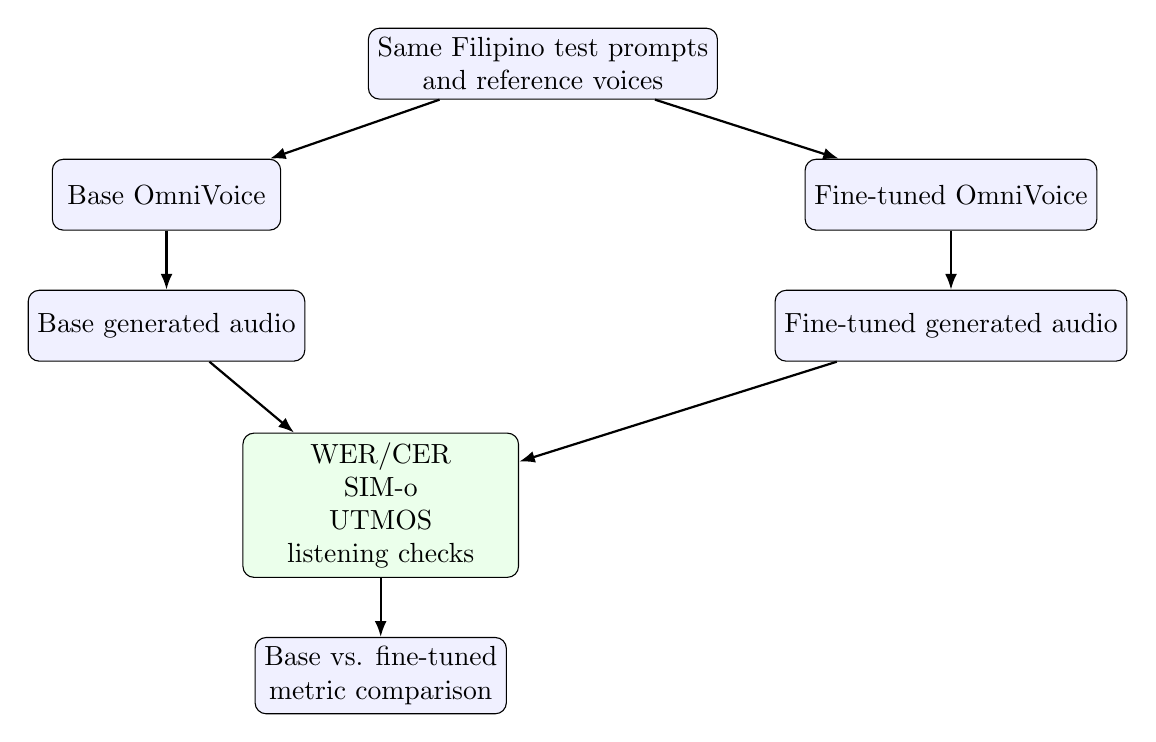
\begin{tikzpicture}[
    node distance=0.75cm and 1.1cm,
    box/.style={draw, rounded corners, align=center, minimum height=0.9cm, minimum width=2.9cm, fill=blue!6},
    metric/.style={draw, rounded corners, align=center, minimum height=0.9cm, minimum width=3.5cm, fill=green!8},
    arrow/.style={-{Latex[length=2mm]}, thick}
  ]
    \node[box] (test) {Same Filipino test prompts\\and reference voices};
    \node[box, below left=of test] (base) {Base OmniVoice};
    \node[box, below right=of test] (fine) {Fine-tuned OmniVoice};
    \node[box, below=of base] (baseaudio) {Base generated audio};
    \node[box, below=of fine] (fineaudio) {Fine-tuned generated audio};
    \node[metric, below right=0.9cm and -0.8cm of baseaudio] (metrics) {WER/CER\\SIM-o\\UTMOS\\listening checks};
    \node[box, below=of metrics] (compare) {Base vs. fine-tuned\\metric comparison};

    \draw[arrow] (test) -- (base);
    \draw[arrow] (test) -- (fine);
    \draw[arrow] (base) -- (baseaudio);
    \draw[arrow] (fine) -- (fineaudio);
    \draw[arrow] (baseaudio) -- (metrics);
    \draw[arrow] (fineaudio) -- (metrics);
    \draw[arrow] (metrics) -- (compare);
  \end{tikzpicture}
\end{figure}

\subsection{Evaluation Metrics}

The evaluation uses three objective metrics from modern zero-shot TTS evaluation: WER/CER for intelligibility, SIM-o for speaker similarity, and UTMOS for naturalness. Because each metric depends on a particular evaluator model or preprocessing pipeline, all evaluation runs use the same test split, inference settings, evaluator checkpoints, and text normalization before comparing base and fine-tuned results.

\subsubsection{Word Error Rate and Character Error Rate}

Word error rate (WER) measures whether the generated speech communicates the intended text. The generated waveform is first transcribed by an automatic speech recognition (ASR) model. The ASR transcript is then compared with the ground-truth target text using edit-distance operations: substitutions ($S$), deletions ($D$), and insertions ($I$). These edit operations trace back to Levenshtein distance \citep{levenshtein}. WER is computed as:

\begin{equation}
  \mathrm{WER} = \frac{S + D + I}{N} \times 100,
\end{equation}

where $N$ is the number of words in the reference text. Lower WER indicates that the ASR system recognized the generated speech as closer to the intended sentence. Character error rate (CER) follows the same idea but computes edit operations over characters instead of words, which can be useful for languages or text-normalization settings where word segmentation affects the metric.

In TTS evaluation, WER is not just a mathematical string distance; it is also dependent on the ASR model used to transcribe generated audio. The OmniVoice evaluation documentation reports different WER backends by benchmark: HuBERT-based WER for LibriSpeech-PC, Whisper for English Seed-TTS, Paraformer for Chinese Seed-TTS, Omnilingual-ASR for FLEURS, and Whisper or Paraformer for MiniMax multilingual evaluation depending on language \citep{omnivoice,hubert,whisper,paraformer}. For this Filipino evaluation, the notebook uses the OmniVoice MiniMax multilingual WER path with Whisper-large-v3 for the non-Chinese Filipino setting and logs insertion, deletion, substitution, and total-word counts. This makes WER useful for comparing base and fine-tuned Filipino outputs, but the result should still be interpreted as ASR-mediated intelligibility rather than a direct human comprehension score.

\subsubsection{Objective Speaker Similarity}

SIM-o measures whether generated speech preserves the voice identity of the reference prompt. Voicebox popularized reporting objective similarity alongside listener-based speaker similarity for zero-shot TTS evaluation \citep{voicebox}. OmniVoice follows the same evaluation family and reports SIM-o as an objective speaker-similarity metric \citep{omnivoice}.

Computationally, SIM-o is the cosine similarity between speaker embeddings extracted from the reference audio and generated audio:

\begin{equation}
  \mathrm{SIM\text{-}o}(r,g) =
  \frac{\mathbf{e}_r \cdot \mathbf{e}_g}
       {\lVert \mathbf{e}_r \rVert \lVert \mathbf{e}_g \rVert},
\end{equation}

where $\mathbf{e}_r$ is the speaker embedding of the reference prompt and $\mathbf{e}_g$ is the speaker embedding of the generated speech. Higher values indicate that the generated speech is closer to the reference speaker in the embedding space.

The reliability of SIM-o depends on the speaker encoder. The OmniVoice evaluation path uses WavLM-based ECAPA-TDNN speaker embeddings. ECAPA-TDNN is a speaker verification architecture that improves TDNN-style speaker embeddings with channel attention, propagation, and aggregation mechanisms \citep{ecapatdnn}. WavLM provides self-supervised speech representations that are useful beyond ASR, including speaker-related tasks \citep{wavlm}. In this study, SIM-o is used to check whether Filipino fine-tuning improves intelligibility without damaging voice cloning identity. A fine-tuned model that reduces WER but lowers SIM-o substantially may be clearer but worse at preserving the reference speaker.

\subsubsection{UTMOS}

UTMOS estimates speech naturalness using a learned mean opinion score (MOS) prediction model. \citet{utmos} introduced UTMOS as the UTokyo-SaruLab system for the VoiceMOS Challenge 2022, where the goal was to predict human MOS ratings for speech samples. Unlike WER, which evaluates textual intelligibility, and SIM-o, which evaluates speaker identity, UTMOS estimates whether the generated waveform sounds natural or human-like.

In the evaluation pipeline, each generated audio file is passed to the UTMOS model, and the resulting predicted MOS values are averaged for each system. Higher UTMOS indicates better predicted naturalness. However, UTMOS is still a predictor trained from listening-test data, so it should not be treated as a complete replacement for human listening checks. For this reason, UTMOS is interpreted together with WER, SIM-o, and selected Filipino listening samples. For example, a model may obtain a high UTMOS score because the waveform is smooth while still mispronouncing Filipino words; conversely, a model may improve WER while sounding less natural.

\subsubsection{Metric Reliability and Results}

The most reliable comparison is a controlled within-study comparison rather than an absolute claim of model quality. Both base and fine-tuned models are evaluated on the same Filipino test prompts, reference voices, inference parameters, ASR model, speaker encoder, UTMOS checkpoint, and text normalization rules. Weights and Biases stores the metric summaries, raw metric logs, generated audio examples, and checkpoint metadata. This makes it possible to compare hyperparameter runs by both development loss and downstream audio metrics.

\begin{table}[H]
  \centering
  \caption{Full PLD Filipino test-set objective results. Lower WER is better; higher SIM-o and UTMOS are better.}
  \small
  \begin{tabular}{p{0.31\linewidth}p{0.22\linewidth}rrrr}
    \toprule
    Model & Selection & WER (\%) & $\Delta$WER & SIM-o & UTMOS \\
    \midrule
    Base OmniVoice & pretrained base & 22.55 & 0.00 & 0.602 & 3.64 \\
    Fine-tuned, 1000 steps, lr 2e-5 & checkpoint-1000 & 20.07 & -2.48 & 0.610 & 3.60 \\
    Fine-tuned, 2000 steps, lr 5e-6 & checkpoint-2000 & 22.64 & +0.09 & 0.611 & 3.57 \\
    Fine-tuned, lr 1e-5 & best eval loss at step 4900 & 18.52 & -4.03 & 0.604 & 3.61 \\
    \bottomrule
  \end{tabular}
  \label{tab:objective-results}
\end{table}

Table~\ref{tab:objective-results} shows that fine-tuning can improve Filipino intelligibility, but not every fine-tuning run improves the downstream metrics. The 1000-step checkpoint reduced WER from 22.55\% to 20.07\%, while increasing SIM-o from 0.602 to 0.610 and lowering UTMOS slightly from 3.64 to 3.60. The 2000-step checkpoint trained with a lower learning rate of 5e-6 achieved the highest SIM-o at 0.611, but its WER rose to 22.64\%, slightly worse than the base model. This indicates that better speaker similarity alone is not enough to identify the best model for this research question.

The strongest checkpoint is the 1e-5 run selected by best development loss at step 4900. It reduced WER to 18.52\%, a 4.03 absolute point improvement over the base model and about a 17.9\% relative WER reduction. Its SIM-o of 0.604 remains slightly above the base model, while its UTMOS of 3.61 is lower than the base model but close to the other fine-tuned checkpoints. Therefore, the best current model is the best-development-loss checkpoint because it gives the largest intelligibility improvement without a large speaker-similarity or naturalness collapse.

\begin{table}[H]
  \centering
  \caption{WER edit-operation counts on the full PLD Filipino test set.}
  \small
  \begin{tabular}{lrrrr}
    \toprule
    Model & Insertions & Deletions & Substitutions & Words \\
    \midrule
    Base OmniVoice & 2,668 & 640 & 2,858 & 27,342 \\
    Fine-tuned, 1000 steps & 2,439 & 598 & 2,452 & 27,354 \\
    Fine-tuned, 2000 steps & 3,115 & 586 & 2,492 & 27,354 \\
    Fine-tuned, best checkpoint & 2,045 & 603 & 2,417 & 27,354 \\
    \bottomrule
  \end{tabular}
  \label{tab:wer-counts}
\end{table}

The edit-operation counts in Table~\ref{tab:wer-counts} help explain the model ranking. The best checkpoint substantially reduces insertions and substitutions relative to the base model. In contrast, the 2000-step checkpoint lowers deletions and substitutions but increases insertions enough to lose the WER improvement.

\begin{thebibliography}{99}

\bibitem[Azzuni and El Saddik(2025)]{voicecloningsurvey}
Azzuni, H., and El Saddik, A. (2025). Voice cloning: Comprehensive survey. \textit{arXiv preprint arXiv:2505.00579}. \url{https://arxiv.org/abs/2505.00579}

\bibitem[Wang et al.(2023)]{valle}
Wang, C., Chen, S., Wu, Y., Zhang, Z., Zhou, L., Liu, S., Chen, Z., Liu, Y., Wang, H., Li, J., He, L., Zhao, S., and Wei, F. (2023). Neural codec language models are zero-shot text to speech synthesizers. \textit{arXiv preprint arXiv:2301.02111}. \url{https://arxiv.org/abs/2301.02111}

\bibitem[Le et al.(2023)]{voicebox}
Le, M., Vyas, A., Shi, B., Karrer, B., Sari, L., Moritz, R., Williamson, M., Manohar, V., Adi, Y., Mahadeokar, J., et al. (2023). Voicebox: Text-guided multilingual universal speech generation at scale. \textit{Advances in Neural Information Processing Systems}, 36, 14005--14034. \url{https://arxiv.org/abs/2306.15687}

\bibitem[Wang et al.(2024)]{maskgct}
Wang, Y., Zhan, H., Liu, L., Zeng, R., Guo, H., Zheng, J., Zhang, Q., Zhang, X., Zhang, S., and Wu, Z. (2024). MaskGCT: Zero-shot text-to-speech with masked generative codec transformer. \textit{arXiv preprint arXiv:2409.00750}. \url{https://arxiv.org/abs/2409.00750}

\bibitem[Chen et al.(2024)]{f5tts}
Chen, Y., Niu, Z., Ma, Z., Deng, K., Wang, C., Zhao, J., Yu, K., and Chen, X. (2024). F5-TTS: A fairytaler that fakes fluent and faithful speech with flow matching. \textit{arXiv preprint arXiv:2410.06885}. \url{https://arxiv.org/abs/2410.06885}

\bibitem[Zhu et al.(2026)]{omnivoice}
Zhu, H., Ye, L., Kang, W., Yao, Z., Guo, L., Kuang, F., Han, Z., Zhuang, W., Lin, L., and Povey, D. (2026). OmniVoice: Towards omnilingual zero-shot text-to-speech with diffusion language models. \textit{arXiv preprint arXiv:2604.00688}. \url{https://arxiv.org/abs/2604.00688}

\bibitem[Boson AI(2025)]{higgsaudio}
Boson AI. (2025). Higgs Audio V2: Redefining expressiveness in audio generation. GitHub repository and release blog. \url{https://github.com/boson-ai/higgs-audio}

\bibitem[Cajote et al.(2024)]{pld}
Cajote, R. D., Guevara, R. C. L., Bayona, M. G. A. R., and Lucas, C. R. G. (2024). Philippine Languages Database: A multilingual speech corpora for developing systems for Philippine spoken languages. \textit{Proceedings of SIGUL 2024}, 264--271. \url{https://aclanthology.org/2024.sigul-1.32/}

\bibitem[Pan and Yang(2010)]{transferlearning}
Pan, S. J., and Yang, Q. (2010). A survey on transfer learning. \textit{IEEE Transactions on Knowledge and Data Engineering}, 22(10), 1345--1359. \url{https://doi.org/10.1109/TKDE.2009.191}

\bibitem[Levenshtein(1966)]{levenshtein}
Levenshtein, V. I. (1966). Binary codes capable of correcting deletions, insertions and reversals. \textit{Soviet Physics Doklady}, 10, 707--710.

\bibitem[Radford et al.(2022)]{whisper}
Radford, A., Kim, J. W., Xu, T., Brockman, G., McLeavey, C., and Sutskever, I. (2022). Robust speech recognition via large-scale weak supervision. \textit{arXiv preprint arXiv:2212.04356}. \url{https://arxiv.org/abs/2212.04356}

\bibitem[Hsu et al.(2021)]{hubert}
Hsu, W.-N., Bolte, B., Tsai, Y.-H. H., Lakhotia, K., Salakhutdinov, R., and Mohamed, A. (2021). HuBERT: Self-supervised speech representation learning by masked prediction of hidden units. \textit{IEEE/ACM Transactions on Audio, Speech, and Language Processing}, 29, 3451--3460. \url{https://arxiv.org/abs/2106.07447}

\bibitem[Gao et al.(2022)]{paraformer}
Gao, Z., Zhang, S., McLoughlin, I., and Yan, Z. (2022). Paraformer: Fast and accurate parallel transformer for non-autoregressive end-to-end speech recognition. \textit{Proceedings of Interspeech 2022}. \url{https://arxiv.org/abs/2206.08317}

\bibitem[Desplanques et al.(2020)]{ecapatdnn}
Desplanques, B., Thienpondt, J., and Demuynck, K. (2020). ECAPA-TDNN: Emphasized channel attention, propagation and aggregation in TDNN based speaker verification. \textit{Proceedings of Interspeech 2020}. \url{https://arxiv.org/abs/2005.07143}

\bibitem[Chen et al.(2021)]{wavlm}
Chen, S., Wang, C., Chen, Z., Wu, Y., Liu, S., Chen, Z., Li, J., Kanda, N., Yoshioka, T., Xiao, X., et al. (2021). WavLM: Large-scale self-supervised pre-training for full stack speech processing. \textit{IEEE Journal of Selected Topics in Signal Processing}, 16(6), 1505--1518. \url{https://arxiv.org/abs/2110.13900}

\bibitem[Saeki et al.(2022)]{utmos}
Saeki, T., Xin, D., Nakata, W., Koriyama, T., Takamichi, S., and Saruwatari, H. (2022). UTMOS: UTokyo-SaruLab system for VoiceMOS Challenge 2022. \textit{Proceedings of Interspeech 2022}. \url{https://arxiv.org/abs/2204.02152}

\bibitem[Rajbhandari et al.(2019)]{zero}
Rajbhandari, S., Rasley, J., Ruwase, O., and He, Y. (2019). ZeRO: Memory optimizations toward training trillion parameter models. \textit{arXiv preprint arXiv:1910.02054}. \url{https://arxiv.org/abs/1910.02054}

\bibitem[Biewald(2020)]{wandb}
Biewald, L. (2020). Experiment tracking with Weights and Biases. Software available from Weights and Biases. \url{https://www.wandb.com/}

\end{thebibliography}

\end{document}
